\section{Results}

\subsection{Main full-scale comparison}

Table~\ref{tab:main-results} reports macro means across the four forecast horizons.

\begin{table*}[t]
\centering
\small
\resizebox{\textwidth}{!}{%
\begin{tabular}{lccccc}
\toprule
Model & Top1 & Top5 & NLL & Brier & ECE \\
\midrule
Markov baseline & 0.3184 & 0.7587 & 2.2788 & 0.8111 & 0.0323 \\
Hierarchical GRU & 0.6648 & 0.9631 & 1.0214 & 0.4578 & 0.0180 \\
TrAISformer-H3 & 0.6803 & 0.9697 & 0.9556 & 0.4361 & 0.0094 \\
FlightBERT++-H3 & 0.6764 & 0.9671 & 0.9791 & 0.4417 & \textbf{0.0086} \\
Transformer horizon decoder & 0.6744 & 0.9656 & 0.9946 & 0.4447 & 0.0123 \\
Multiscale Transformer & 0.6827 & 0.9685 & 0.9641 & 0.4338 & 0.0093 \\
\textbf{Horizon-Router} & \textbf{0.6884} & \textbf{0.9710} & \textbf{0.9399} & \textbf{0.4262} & 0.0104 \\
\bottomrule
\end{tabular}

}
\caption{Macro-mean full-scale comparison across 10, 30, 60, and 120 minute horizons.}
\label{tab:main-results}
\end{table*}

\begin{figure}[!t]
\centering
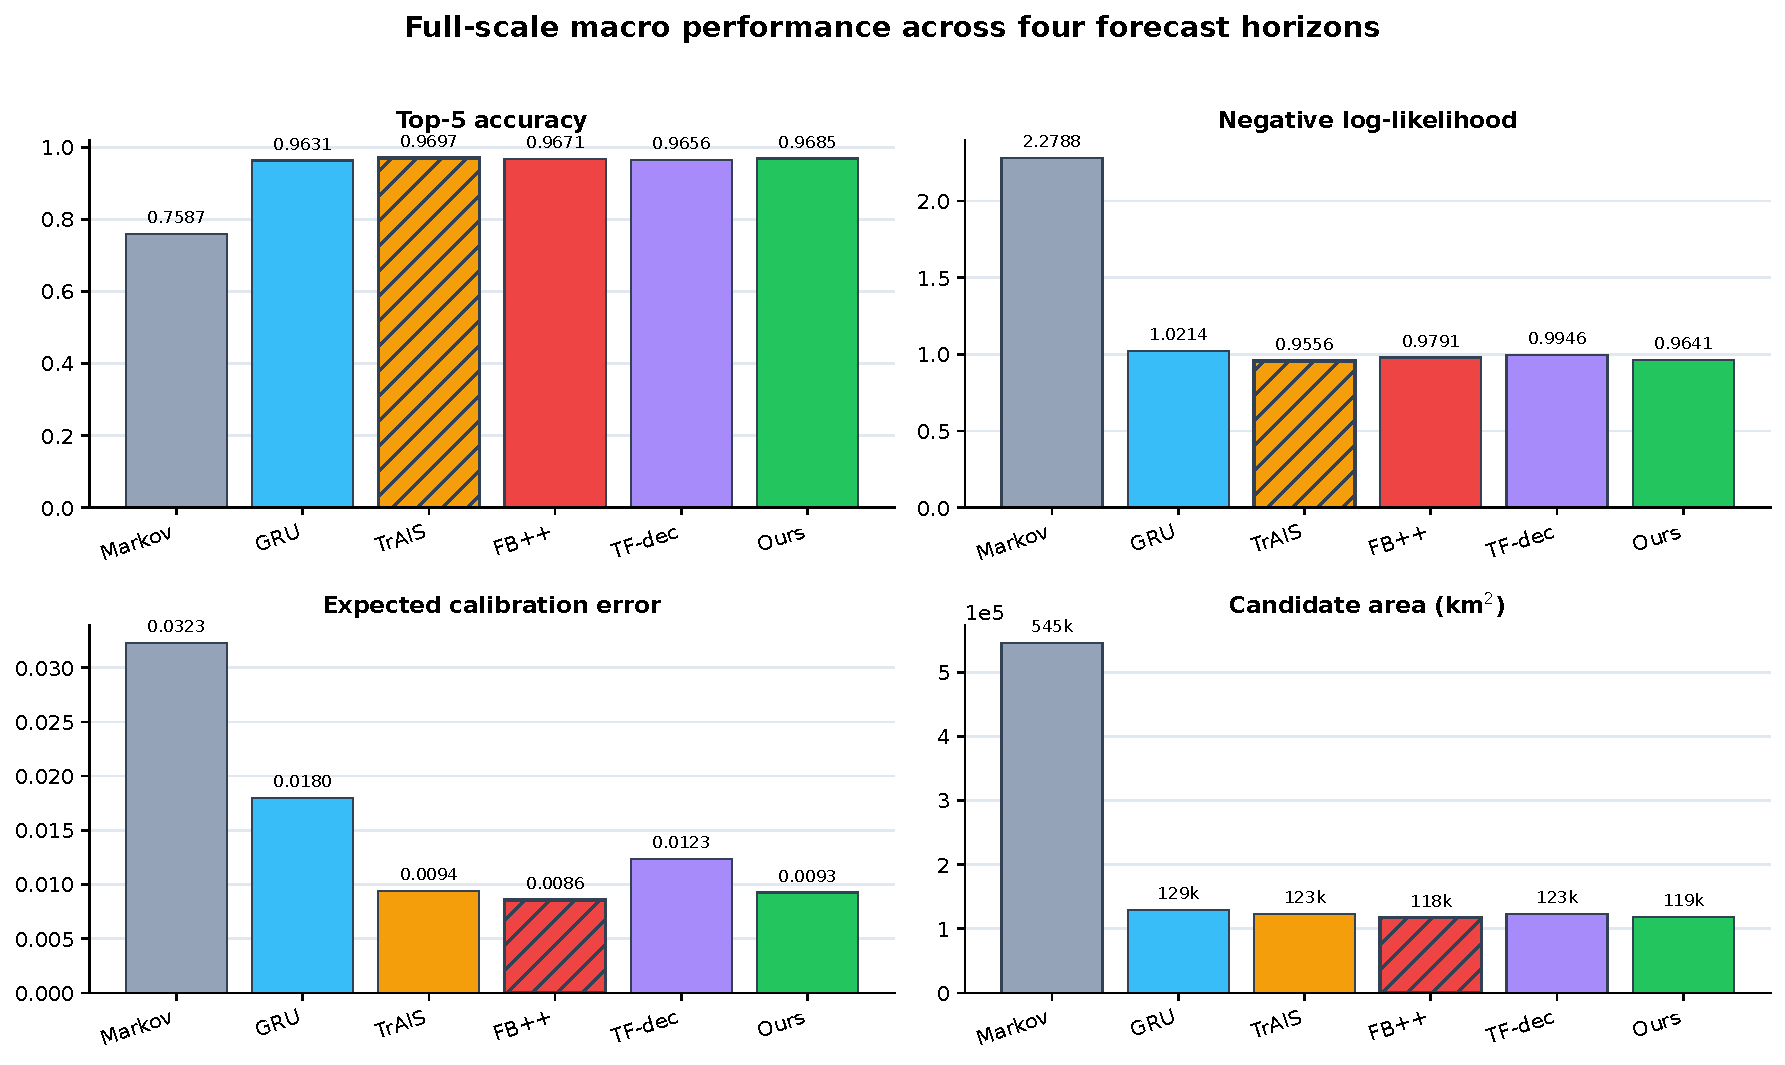
\includegraphics[width=\textwidth]{figures/fig2_main_results_overview.pdf}
\caption{Main full-scale result overview. Relative to internal baselines and two adapted external baselines, the proposed multiscale model provides the strongest balance between top-1 accuracy, probability quality, and candidate-set compactness.}
\label{fig:main-results-overview}
\end{figure}

Three observations stand out. First, all learned hierarchical models strongly outperform the classical Markov baseline. Second, among the two adapted external baselines, TrAISformer-H3 is the strongest competitor: it attains the best macro top-3/top-5, the lowest NLL, and the highest union cover. Third, the proposed multiscale model still achieves the best macro top-1 (0.6827), the best Brier score (0.4338), and the smallest candidate union cell count (2.1829), which makes it the most balanced method in terms of correctness, probabilistic quality, and candidate compactness.

FlightBERT++-H3 exhibits a different trade-off. It obtains the lowest macro ECE (0.0086) and the smallest candidate union area (117,593 km$^2$), but it remains behind the proposed model on top-1/top-3/top-5 and union cover. This indicates that tighter and more conservative candidate sets do not automatically translate into better regional forecasting when ranking quality weakens.

The per-horizon results also clarify where the multiscale design matters. TrAISformer-H3 is slightly stronger on top-3/top-5 at 10 and 30 minutes, but the proposed model regains a clear advantage at 120 minutes: top-1 rises from 0.5481 to 0.5565, top-3 from 0.8482 to 0.8531, and top-5 from 0.9355 to 0.9372, while NLL, Brier, and ECE all improve as well. This supports our central claim that explicit multiscale temporal modeling contributes most strongly to medium- and long-horizon regional forecasting rather than only improving short-horizon ranking metrics.

\subsection{Improvements over the hierarchical GRU baseline}

Against the hierarchical GRU baseline, the proposed model improves all top-k metrics and all probabilistic metrics: top-1 from 0.6648 to 0.6827, top-3 from 0.9076 to 0.9174, top-5 from 0.9631 to 0.9685, NLL from 1.0214 to 0.9641, Brier from 0.4578 to 0.4338, and ECE from 0.0180 to 0.0093.

The gain is consistent across horizons. Table~\ref{tab:delta-gru} shows horizon-wise differences relative to the GRU baseline.

\begin{table}[t]
\centering
\small
\resizebox{\columnwidth}{!}{%
\begin{tabular}{ccccccccc}
\toprule
Horizon & $\Delta$Top1 & $\Delta$Top3 & $\Delta$Top5 & $\Delta$NLL & $\Delta$Brier & $\Delta$ECE & $\Delta$Cover@Budget & $\Delta$Union Area km$^2$ \\
\midrule
10m & +0.0199 & +0.0059 & +0.0031 & -0.0516 & -0.0281 & -0.0085 & +0.0001 & -2316 \\
30m & +0.0214 & +0.0129 & +0.0076 & -0.0759 & -0.0303 & -0.0210 & +0.0006 & -4567 \\
60m & +0.0115 & +0.0054 & +0.0018 & -0.0340 & -0.0158 & -0.0016 & +0.0001 & -7705 \\
120m & +0.0190 & +0.0153 & +0.0091 & -0.0674 & -0.0220 & -0.0040 & +0.0004 & -26031 \\
\bottomrule
\end{tabular}

}
\caption{Per-horizon delta of the proposed model relative to the hierarchical GRU baseline. Positive is better for top-k and union cover; negative is better for NLL, Brier, ECE, candidate cells, and candidate area.}
\label{tab:delta-gru}
\end{table}

\subsection{Structural ablation: is the multiscale branch necessary?}

To isolate the value of explicit multiscale temporal encoding, we compare the final model with a single-scale Transformer horizon decoder that already has horizon-specific queries but no multiscale branch.

\begin{table}[t]
\centering
\small
\resizebox{\columnwidth}{!}{%
\begin{tabular}{lcccccccc}
\toprule
Model & Top1 & Top3 & Top5 & NLL & Brier & ECE & Cover@Budget & Union Area km$^2$ \\
\midrule
Transformer horizon decoder & 0.6744 & 0.9129 & 0.9656 & 0.9946 & 0.4447 & 0.0123 & 0.9981 & 122553 \\
\textbf{Proposed multiscale model} & \textbf{0.6827} & \textbf{0.9174} & \textbf{0.9685} & \textbf{0.9641} & \textbf{0.4338} & \textbf{0.0093} & \textbf{0.9983} & \textbf{118810} \\
\bottomrule
\end{tabular}

}
\caption{Structural ablation comparing the single-scale Transformer horizon decoder with the proposed multiscale model.}
\label{tab:structural-ablation}
\end{table}

The multiscale branch improves every main macro metric and also reaches a lower validation loss (0.3055 vs. 0.3177). This supports the claim that explicit dual-scale temporal modeling adds value beyond simply replacing the GRU with a Transformer.

\subsection{H3-neighbor refinement is a recall-versus-calibration trade-off}

We next evaluate H3-neighbor refinement with three diffusion strengths. The refinement improves probability-mass candidate recall, but it is not a free gain.

\begin{table}[t]
\centering
\small
\resizebox{\columnwidth}{!}{%
\begin{tabular}{lccccccc}
\toprule
Model & Top5 & NLL & Brier & ECE & Cover@Budget & Union Area km$^2$ & Union Cover \\
\midrule
Final model & \textbf{0.9685} & 0.9641 & \textbf{0.4338} & \textbf{0.0093} & 0.9983 & \textbf{118810} & 0.8922 \\
Refine a=0.05 & 0.9677 & \textbf{0.9593} & 0.4344 & 0.0310 & \textbf{0.9987} & 127062 & 0.9052 \\
Refine a=0.10 & 0.9673 & 0.9796 & 0.4372 & 0.0585 & 0.9987 & 137220 & 0.9192 \\
Refine a=0.20 & 0.9662 & 1.0340 & 0.4493 & 0.1135 & 0.9987 & 167889 & \textbf{0.9496} \\
\bottomrule
\end{tabular}

}
\caption{H3-neighbor refinement sweep on the full dataset. Higher union cover comes with worse calibration and larger candidate sets.}
\label{tab:h3-refine}
\end{table}

\begin{figure}[t]
\centering
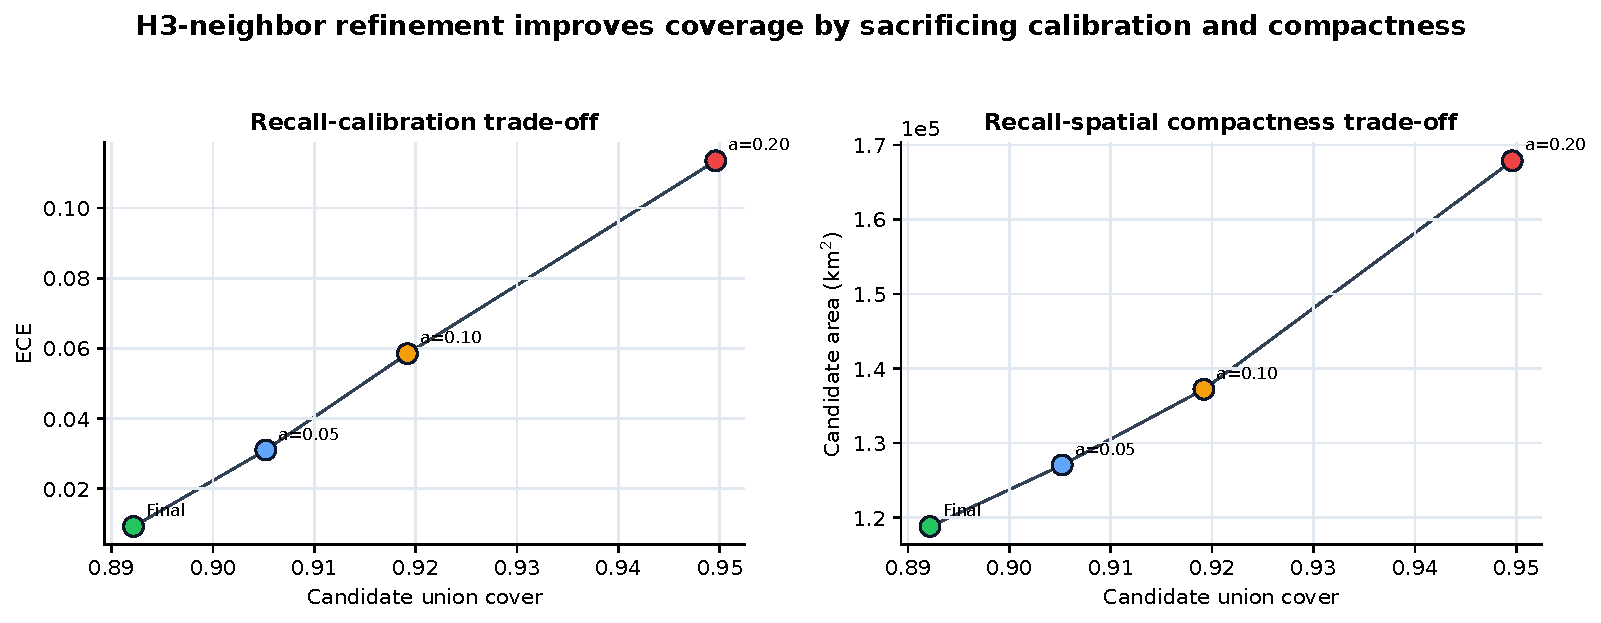
\includegraphics[width=\columnwidth]{figures/fig3_h3_refinement_tradeoff.pdf}
\caption{H3-neighbor refinement increases candidate union coverage, but the added recall comes with worse calibration and larger spatial candidate areas.}
\label{fig:h3-refinement-tradeoff}
\end{figure}

The refinement increases candidate union cover, but it quickly degrades calibration and eventually worsens top-5 and NLL. Therefore, it should not be presented as the final model. Its value lies in exposing a useful operational trade-off: local spatial smoothing can improve recall, but only by sacrificing confidence quality and spatial compactness.

\subsection{Reachability filtering has a small aggregate effect}

Turning reachability filtering off produces only very small aggregate metric changes. This suggests that, in the present setup, reachability filtering acts more as a plausibility safeguard than as the primary source of predictive gains.
